\begin{minipage}{0.75\linewidth}
\begin{figure}[h]
    \centering
    \begin{adjustbox}{max width=1.0\linewidth, keepaspectratio}
        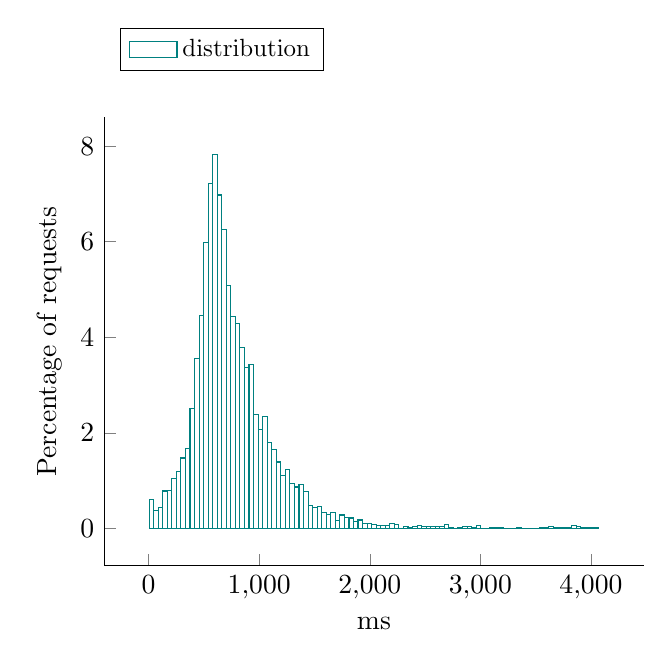
\begin{tikzpicture}
            \begin{axis}[ylabel = Percentage of requests, 
xlabel = ms, 
legend style = {nodes={scale=0.9, transform shape}, at={(0.03,1.2)}, anchor=north west, draw=black, fill=white, align=left, legend columns=3},
area style, mark size = 0pt,
 cycle list name = exotic,
  axis lines* = left]
		\addplot +[ybar interval] coordinates {
			 (4, 0.596953)
			 (45.08, 0.370523)
			 (86.16, 0.432277)
			 (127.24, 0.782215)
			 (168.32, 0.792507)
			 (209.4, 1.03952)
			 (250.48, 1.19391)
			 (291.56, 1.4718)
			 (332.64, 1.66735)
			 (373.72, 2.50103)
			 (414.8, 3.56114)
			 (455.88, 4.44627)
			 (496.96, 5.97983)
			 (538.04, 7.2149)
			 (579.12, 7.82215)
			 (620.2, 6.97818)
			 (661.28, 6.24743)
			 (702.36, 5.0844)
			 (743.44, 4.42569)
			 (784.52, 4.2816)
			 (825.6, 3.77727)
			 (866.68, 3.37587)
			 (907.76, 3.42734)
			 (948.84, 2.38781)
			 (989.92, 2.06875)
			 (1031, 2.34664)
			 (1072.08, 1.80115)
			 (1113.16, 1.65706)
			 (1154.24, 1.38946)
			 (1195.32, 1.11157)
			 (1236.4, 1.22478)
			 (1277.48, 0.946892)
			 (1318.56, 0.864553)
			 (1359.64, 0.916015)
			 (1400.72, 0.771923)
			 (1441.8, 0.473446)
			 (1482.88, 0.442569)
			 (1523.96, 0.452861)
			 (1565.04, 0.329354)
			 (1606.12, 0.288184)
			 (1647.2, 0.339646)
			 (1688.28, 0.164677)
			 (1729.36, 0.277892)
			 (1770.44, 0.226431)
			 (1811.52, 0.216138)
			 (1852.6, 0.1338)
			 (1893.68, 0.174969)
			 (1934.76, 0.102923)
			 (1975.84, 0.102923)
			 (2016.92, 0.0720461)
			 (2058, 0.0514615)
			 (2099.08, 0.0617538)
			 (2140.16, 0.0514615)
			 (2181.24, 0.0926307)
			 (2222.32, 0.0720461)
			 (2263.4, 0)
			 (2304.48, 0.0308769)
			 (2345.56, 0.0205846)
			 (2386.64, 0.0308769)
			 (2427.72, 0.0617538)
			 (2468.8, 0.0411692)
			 (2509.88, 0.0308769)
			 (2550.96, 0.0308769)
			 (2592.04, 0.0411692)
			 (2633.12, 0.0308769)
			 (2674.2, 0.0823384)
			 (2715.28, 0.0205846)
			 (2756.36, 0)
			 (2797.44, 0.0205846)
			 (2838.52, 0.0308769)
			 (2879.6, 0.0308769)
			 (2920.68, 0.0205846)
			 (2961.76, 0.0514615)
			 (3002.84, 0)
			 (3043.92, 0)
			 (3085, 0.0205846)
			 (3126.08, 0.0102923)
			 (3167.16, 0.0102923)
			 (3208.24, 0)
			 (3249.32, 0)
			 (3290.4, 0)
			 (3331.48, 0.0205846)
			 (3372.56, 0)
			 (3413.64, 0)
			 (3454.72, 0)
			 (3495.8, 0)
			 (3536.88, 0.0102923)
			 (3577.96, 0.0102923)
			 (3619.04, 0.0308769)
			 (3660.12, 0.0205846)
			 (3701.2, 0.0205846)
			 (3742.28, 0.0102923)
			 (3783.36, 0.0102923)
			 (3824.44, 0.0617538)
			 (3865.52, 0.0308769)
			 (3906.6, 0.0205846)
			 (3947.68, 0.0102923)
			 (3988.76, 0.0102923)
			 (4029.84, 0.0102923)
			 (4070.92, 0.0102923)
		};
\addlegendentry{distribution};
           \end{axis}
      \end{tikzpicture}
  \end{adjustbox}
  \caption{Response time distribution - req = ReadUser-2}
\end{figure}
\end{minipage}\hfill\begin{minipage}{0.18\linewidth}
\begin{table}[h]
\begin{tabular}{|cc|}
\hline
\textbf{} & \textbf{ms}\\ \hline
 \Xhline{0.005\arrayrulewidth}
min & 4\\
 \Xhline{0.005\arrayrulewidth}
max & 4112\\
 \Xhline{0.005\arrayrulewidth}
mean & 768\\
 \Xhline{0.005\arrayrulewidth}
std & 405\\
\hline
\hline
 \Xhline{0.005\arrayrulewidth}
25th & 540\\
 \Xhline{0.005\arrayrulewidth}
50th & 682\\
 \Xhline{0.005\arrayrulewidth}
75th & 920\\
 \Xhline{0.005\arrayrulewidth}
80th & 993\\
 \Xhline{0.005\arrayrulewidth}
85th & 1089\\
 \Xhline{0.005\arrayrulewidth}
90th & 1226\\
 \Xhline{0.005\arrayrulewidth}
95th & 1446\\
 \Xhline{0.005\arrayrulewidth}
99th & 2212\\
\hline
\end{tabular}
\caption{Response time}
\end{table}
\end{minipage}\hfill